\documentclass[serif, aspectratio=169]{beamer}
\usepackage[T1]{fontenc} 
\usepackage{fourier}
\usepackage{hyperref}
\usepackage{latexsym,amsmath,xcolor,multicol,booktabs,calligra}
\usepackage{booktabs} % For better table formatting
\usepackage{graphicx,pstricks,listings,stackengine}
\usepackage{listings}
\usepackage{array} 
\usepackage{colortbl}

\author{Dr.Hajialiasgari}
\title{Machine Learning}
\institute{
    Tehran University \\
    Of\\
    Medical Science
}
\date{\small \today}
\usepackage{UoWstyle}

% Define custom colors and styles for listings
\definecolor{deepblue}{rgb}{0,0,0.5}
\definecolor{deepred}{RGB}{153,0,0}
\definecolor{deepgreen}{rgb}{0,0.5,0}
\definecolor{halfgray}{gray}{0.55}

\lstset{
    basicstyle=\ttfamily\small,
    keywordstyle=\bfseries\color{deepblue},
    emphstyle=\ttfamily\color{deepred},
    stringstyle=\color{deepgreen},
    numbers=left,
    numberstyle=\small\color{halfgray},
    rulesepcolor=\color{red!20!green!20!blue!20},
    frame=shadowbox,
}

\begin{document}

\begin{frame}
    \titlepage
    \vspace*{-0.6cm}
    \begin{figure}[htpb]
        \begin{center}
            \includegraphics[keepaspectratio, scale=0.05]{Tumsl-logo.png}
        \end{center}
    \end{figure}
\end{frame}

\begin{frame}    
\tableofcontents[sectionstyle=show, subsectionstyle=show/shaded/hide, subsubsectionstyle=show/shaded/hide]
\end{frame}

\section{Feature Engineering}

\section{Why Feature Engineering is Important?}
\begin{frame}
    \begin{itemize}
        \item Feature engineering is crucial in machine learning as it transforms raw data into meaningful features, enhancing model performance and accuracy. By creating, selecting, and preprocessing features, it helps algorithms better understand patterns, leading to improved predictions and insights.
    \end{itemize}
\end{frame}


\section{A Good Feature...}

\begin{frame}
    \begin{itemize}  
        \item \texttt{\color{red}Relevant:}Directly related to the target variable and contributes to prediction accuracy.  
        \item \texttt{\color{red}Independent:}Minimally correlated with other features to avoid redundancy.  
        \item \texttt{\color{red}Discriminative:} Distinguishes between different classes or outcomes effectively.  
        \item \texttt{\color{red}Robust:} Handles noise, missing values, and outliers without degrading model performance.  
    \end{itemize}
\end{frame}

\section{Different Types of Features}

\begin{frame}
    \begin{itemize}
        \item \texttt{\color{red}Numerical Features:} Quantitative data that represent measurable quantities (e.g., age, salary).
        \item \texttt{\color{red}Categorical Features:} Qualitative data with discrete values representing categories (e.g., gender, city).
        \item \texttt{\color{red}Ordinal Features:} Categorical data with a meaningful order or ranking (e.g., education level: high school, bachelor's, master's).
        \item \texttt{\color{red}Binary Features:} Variables with only two possible values (e.g., 0/1, true/false).
  \end{itemize}

\end{frame}

\begin{frame}
    \begin{itemize}
        \item \texttt{\color{red}Textual Features:} Data in text format requiring techniques like tokenization or embedding (e.g., customer reviews).
        \item \texttt{\color{red}Temporal Features:} Data involving time, such as timestamps or durations (e.g., transaction date).
        \item \texttt{\color{red}Spatial Features:} Data related to location or geography (e.g., latitude and longitude).
        \item \texttt{\color{red}Derived Features:} Features created from raw data using transformations, combinations, or domain knowledge.
    \end{itemize}
\end{frame}

\section{Managing Missing Values}

\begin{frame}{Categorical Features}
    \begin{itemize}
        \item \texttt{\color{green}Imputation with a Constant:} Replace missing values with a placeholder such as \texttt{'Unknown'} or \texttt{'Missing'}. Useful when the absence of data has its own meaning.
        \item \texttt{\color{green}Mode Imputation:} Replace missing values with the most frequent category. Suitable for features with a clear dominant class.
        \item \texttt{\color{green}Imputation Based on Other Features:} Predict missing values using other related features. Requires advanced techniques like regression or classification models.
        \item \texttt{\color{green}Frequency Encoding:} Replace missing values with the frequency or probability of each category.
    \end{itemize}
\end{frame}

\begin{frame}{Categorical Features}
    \begin{itemize}
         \item \texttt{\color{green}Custom Imputation:} Use domain knowledge to assign meaningful values. Effective when the missingness has a known context.
         \item \texttt{\color{green}Separate Category:} Treat missing values as a separate category. Ideal for algorithms that can handle additional classes, such as decision trees.
        \item \texttt{\color{green}Remove Rows/Columns:} Remove data points or features with too many missing values. Only appropriate when the missing data is non-critical or minimal.
    \end{itemize}
\end{frame}

\begin{frame}{Numerical Features}
    \begin{itemize}
         \item \texttt{\color{blue}Mean Imputation:} Replace missing values with the mean of the feature. Works well for data with a normal distribution.
         \item \texttt{\color{blue}Median Imputation:} Replace missing values with the median of the feature. Suitable for skewed data or features with outliers.
         \item \texttt{\color{blue}Mode Imputation:} Replace missing values with the mode (most frequent value). Useful when a single value dominates the feature.
         \item \texttt{\color{blue}Imputation Using Other Features:} Predict missing values using related features through regression or machine learning models. Effective for datasets with strong feature relationships.
    \end{itemize}
\end{frame}

\begin{frame}{Numerical Features}
    \begin{itemize}
         \item \texttt{\color{blue}Interpolation:} Estimate missing values using trends in the data (e.g., linear or polynomial interpolation). Works well for time series or sequential data.
        \item \texttt{\color{blue}Filling with a Constant:} Replace missing values with a specific constant, such as 0. Appropriate when the missing values represent an absence.
        \item \texttt{\color{blue}Remove Rows/Columns:} Drop rows or features with too many missing values. Suitable when the proportion of missing values is high and the feature is non-critical.
        \item \texttt{\color{blue}Use KNN Imputation:} Fill missing values by averaging the values of the \texttt{k}-nearest neighbors. Effective when similar data points are present.
    \end{itemize}
\end{frame}


\section{Calendar Features}

\begin{frame}
    \begin{itemize}
        \item These features are especially beneficial in time-series forecasting, sales analysis, and any context where time plays a significant role in influencing patterns or behaviors.
    \end{itemize}
    
\end{frame}

\begin{frame}
    \begin{itemize}
        \item \texttt{\color{purple}Day of the Week:} Indicates the specific day (e.g., Monday, Tuesday) to capture weekday or weekend effects.
        \item \texttt{\color{purple}Month:} Represents the month (e.g., January, February) to account for seasonal variations.
        \item \texttt{\color{purple}Year:} Useful for capturing long-term trends or changes over years.
        \item \texttt{\color{purple}Quarter:} Denotes the quarter of the year (e.g., Q1, Q2) to capture business cycles or seasonal trends.
        \item \texttt{\color{purple}Day of the Month:} Specifies the day within a month (e.g., 1st, 15th).   
    \end{itemize}
\end{frame}

\begin{frame}
    \begin{itemize}
        \item \texttt{\color{purple}Week of the Year:} Captures the week number in a year (e.g., Week 1, Week 52).
        \item \texttt{\color{purple}Is Weekend/Weekday:} A binary feature indicating whether a date falls on a weekend or a weekday.
        \item \texttt{\color{purple}Is Holiday:} Indicates whether the date is a public or special holiday, often determined based on local calendars.
        \item \texttt{\color{purple}Season:} Classifies the date into a season (e.g., Spring, Summer) to capture climate or activity-based trends.
        \item \texttt{\color{purple}Elapsed Time:} Measures the time difference between the given date and a reference date (e.g., days since a start date).
    \end{itemize}
\end{frame}

\section{Feature Synthesis}

\begin{frame}
    \begin{itemize}
        \item Feature Synthesis in machine learning refers to the process of creating new features by combining or transforming existing ones. 
        \item These synthesized features can capture complex relationships or patterns that may not be explicitly represented in the raw data, thereby improving model performance. It is a part of feature engineering and often requires domain knowledge or automated tools.
    \end{itemize}
\end{frame}

\begin{frame}{Key Techniques for Feature Synthesis}
    \begin{itemize}
        \item \texttt{\color{teal}Mathematical Transformations:}Apply arithmetic operations to existing features.\hfill \textit{Example:}Combine \texttt{length} and \texttt{width} to calculate \texttt{area}.
    
        \item \texttt{\color{teal}Polynomial Features:} Generate higher-order combinations of numerical features.\hfill \textit{Example:} Squaring or cubing features for non-linear modeling.
    
        \item \texttt{\color{teal}Aggregation:} Summarize data across groups using operations like mean, median, or sum.\hfill \textit{Example:} Average transaction value per customer.
    
        \item \texttt{\color{teal}Interaction Features:} Combine features to represent their interaction.\hfill \textit{Example:} Combine \texttt{age} and \texttt{income} to analyze purchasing behavior.
    \end{itemize}  
\end{frame}

\begin{frame}{Key Techniques for Feature Synthesis}
    \begin{itemize}
        \item \texttt{\color{teal}Date/Time-Based Features:} Extract insights from timestamps.\hfill \textit{Example:} Day of the week, quarter, or duration of an event.
    
        \item \texttt{\color{teal}Encoding Categorical Features:} Convert categories into meaningful numerical representations.\hfill \textit{Example:} Frequency or target encoding.
    
        \item \texttt{\color{teal}Text Features:} Extract features from text data using NLP techniques.\hfill \textit{Example:} TF-IDF or sentiment analysis.
    
        \item \texttt{\color{teal}Domain-Specific Features:} Leverage domain knowledge to create relevant features.\hfill \textit{Example:} Calculate BMI in healthcare using weight and height.
    \end{itemize}  
\end{frame}

\section{Feature Scaling}

\begin{frame}{Definition}
    \begin{itemize}
        \item Feature scaling is a preprocessing technique used to normalize or standardize the range of independent features (input variables) in a dataset. It ensures that features contribute equally to the model's performance, avoiding bias toward features with larger scales.
    \end{itemize}
\end{frame}

\begin{frame}{Why is Feature Scaling Important?}
    \begin{itemize}
        \item \texttt{\color{teal}Improves Model Performance:} Many machine learning algorithms, such as gradient descent-based models, perform better when features are scaled consistently.

        \item \texttt{\color{teal}Handles Different Ranges:} Features with vastly different ranges (e.g., income in dollars vs. age in years) can skew the results.

        \item \texttt{\color{teal}Enhances Convergence:} Models like neural networks and SVMs converge faster with scaled features.

        \item \texttt{\color{teal}Reduces Sensitivity to Scale:} Distance-based models (e.g., KNN, K-means) rely on scaled data to calculate accurate distances.
    \end{itemize}
\end{frame}

\begin{frame}{Common Techniques for Feature Scaling}
    \begin{itemize}
        \item \texttt{\color{teal}Min-Max Scaling (Normalization):} Transforms features to a fixed range, typically [0, 1].  
        \begin{itemize}
            \item \textbf{Formula:} 
            \[
            x' = \frac{x - x_{min}}{x_{max} - x_{min}}
            \]
            \item \textbf{Use Case:} Suitable when the data distribution is not Gaussian.
        \end{itemize}

        \item \texttt{\color{teal}Standardization (Z-Score Scaling):} Centers the data around 0 with a standard deviation of 1.  
        \begin{itemize}
            \item \textbf{Formula:} 
            \[
            x' = \frac{x - \mu}{\sigma}
            \]
            \item \textbf{Use Case:} Effective for models requiring Gaussian-like data.
        \end{itemize}
    \end{itemize}
\end{frame}

\section{Data Leakage}

\begin{frame}{Definition}
    \begin{itemize}
        \item Data leakage occurs when information from outside the training dataset is inappropriately used to create a machine learning model, leading to overly optimistic performance metrics during training and poor performance on unseen data.
    \end{itemize}
\end{frame}

\begin{frame}{Why is Data Leakage a Problem?}
    \begin{itemize}
        \item \texttt{\color{teal}Unrealistic Performance Metrics:} The model appears to perform well during training or validation but fails in real-world scenarios.
    
        \item \texttt{\color{teal}Overfitting:} The model relies on leaked information rather than learning true patterns from the data.
    
        \item \texttt{\color{teal}Loss of Generalization:} The model cannot generalize to new, unseen data, rendering it ineffective in production.
    \end{itemize}
\end{frame}

\begin{frame}{Common Causes of Data Leakage}
    \begin{itemize}
        \item \texttt{\color{teal}Target Leakage:} When features contain information about the target that wouldn’t be available during prediction.  
        \textbf{Example:} Using future sales data to predict current sales.

        \item \texttt{\color{teal}Train-Test Contamination:} Test data is used during training, compromising evaluation.  
        \textbf{Example:} Normalizing the entire dataset before splitting.

        \item \texttt{\color{teal}Temporal Leakage:} Using future data to predict past or present outcomes.  
        \textbf{Example:} Including post-event data for event prediction.

        \item \texttt{\color{teal}Improper Cross-Validation:} Data from test folds leaks into training folds during validation.
    \end{itemize}
\end{frame}

\begin{frame}{Cross-Validation}
   \centering
   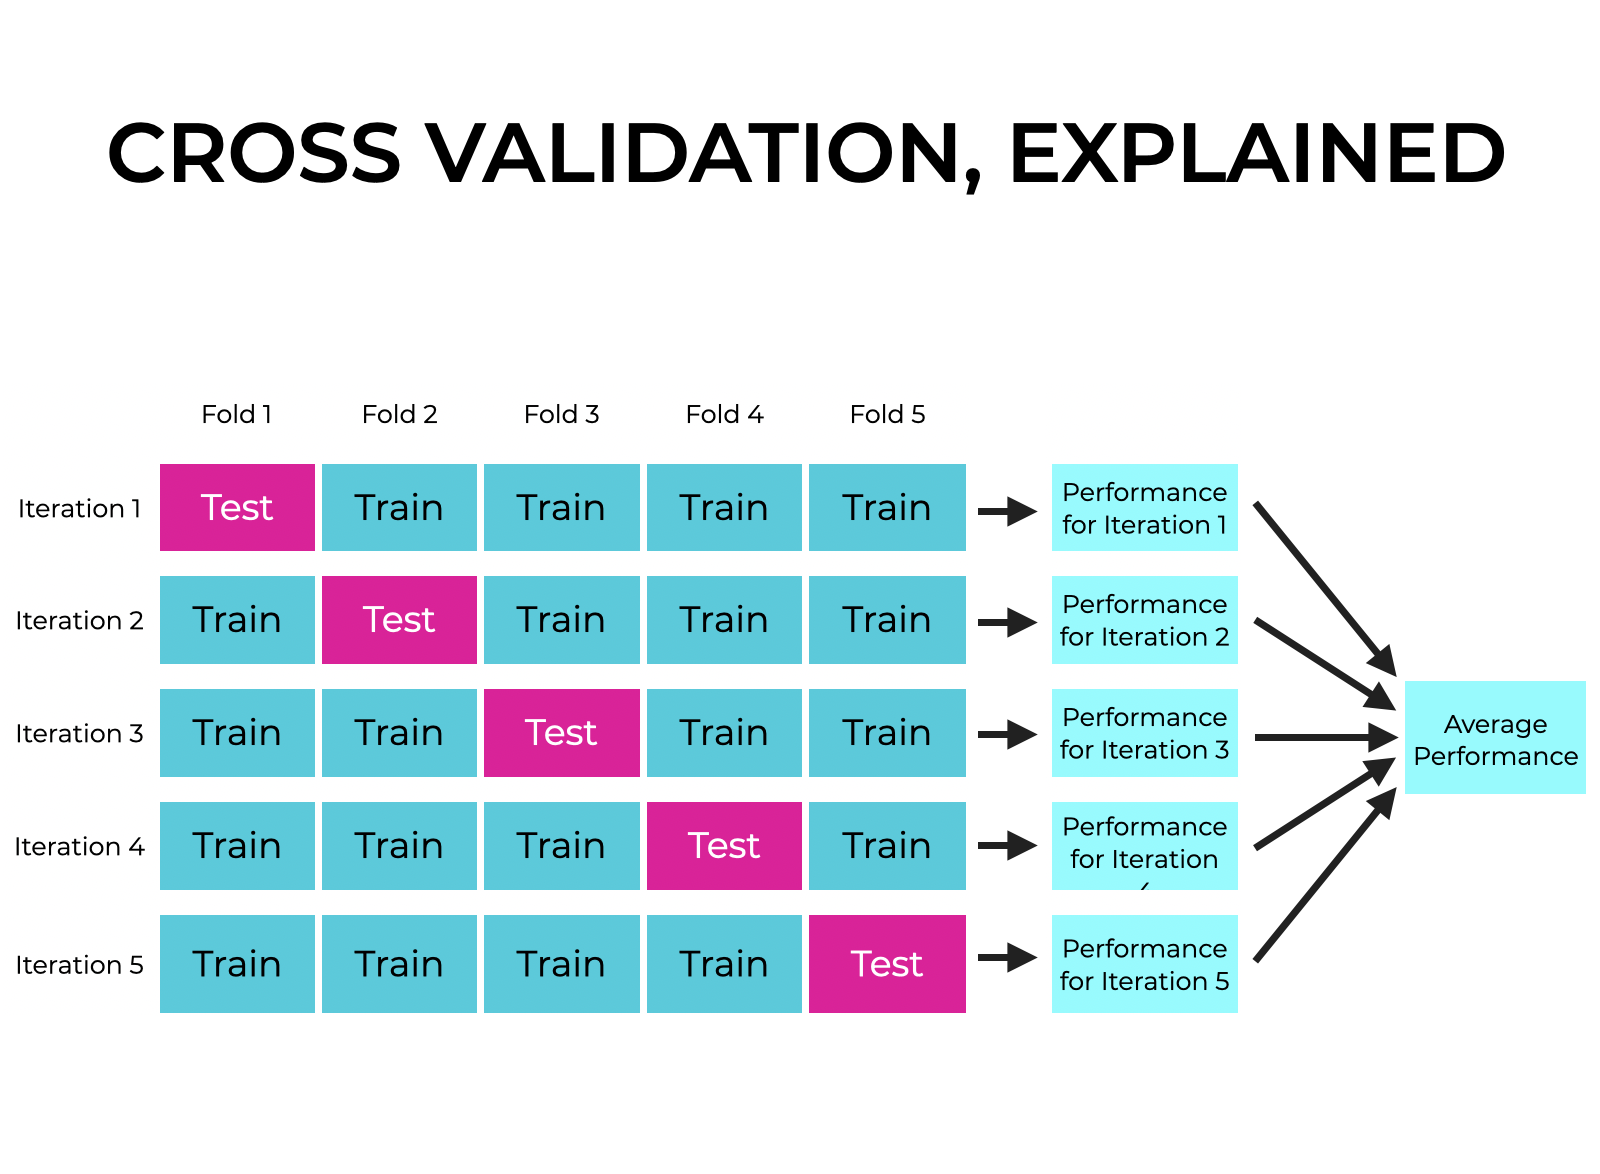
\includegraphics[width=0.8\textwidth]{cross-validation.png}
\end{frame}

\begin{frame}{How to Prevent Data Leakage?}
    \begin{itemize}
        \item \texttt{\color{teal}Careful Feature Selection:} 
        Ensure features do not contain information about the target variable.

        \item \texttt{\color{teal}Correct Data Splitting:} 
        Split the dataset into train, validation, and test sets before any preprocessing.

        \item \texttt{\color{teal}Time-Aware Splitting:} 
        For time-series data, split based on time to avoid future data influencing predictions.

        \item \texttt{\color{teal}Isolation of Test Data:} 
        Keep the test set separate and untouched until the final evaluation.

        \item \texttt{\color{teal}Use of Pipelines:} 
        Automate preprocessing and training to ensure consistent operations across splits.
    \end{itemize}
\end{frame}

\section{Curse of Dimensionality}

\begin{frame}{Definition}
    \begin{itemize}
        \item The curse of dimensionality refers to the challenges and inefficiencies that arise when analyzing and organizing data in high-dimensional spaces. As the number of features (dimensions) increases, the amount of data needed to maintain the same level of performance grows exponentially.
    \end{itemize}
\end{frame}

\begin{frame}{Why is it a Problem?}
     \begin{itemize}
        \item \texttt{\color{teal}Sparse Data in High Dimensions:} As dimensions increase, data points become more spread out, making it difficult for models to find meaningful patterns.

        \item \texttt{\color{teal}Increased Computational Cost:} High-dimensional data requires more memory and computation, slowing down training and prediction.

        \item \texttt{\color{teal}Overfitting Risk:} Models may capture noise instead of meaningful patterns due to the vast feature space.

        \item \texttt{\color{teal}Reduced Model Interpretability:} High-dimensional data makes it harder to understand relationships between features and the target variable.
\end{itemize}
\end{frame}

\begin{frame}{How to Mitigate the Curse of Dimensionality ?}
     \begin{itemize}
         \item \texttt{\color{teal}Feature Selection:} 
         Select only the most relevant features for your model.

         \item \texttt{\color{teal}Dimensionality Reduction:} 
         Use techniques like PCA or t-SNE to reduce the number of dimensions.

        \item \texttt{\color{teal}Regularization Techniques:} 
        Prevent overfitting by adding penalties to complex models.

        \item \texttt{\color{teal}Increase Data Volume:} 
        Gather more data to compensate for the increased feature space.
    \end{itemize}
\end{frame}

\section{Feature Selection}

\begin{frame}{Why is Feature Selection Important?}
    \begin{itemize}
        \item \texttt{\color{teal}Improves Model Performance:} 
        Removes irrelevant features, allowing the model to focus on the most important information, leading to better accuracy.

        \item \texttt{\color{teal}Reduces Overfitting:} 
        Fewer features reduce the risk of the model capturing noise, preventing overfitting.

        \item \texttt{\color{teal}Enhances Generalization:} 
        A simpler model generalizes better to new, unseen data.

        \item \texttt{\color{teal}Reduces Computational Cost:} 
        With fewer features, the model requires less memory and computation, speeding up training.

        \item \texttt{\color{teal}Improves Interpretability:} 
        A model with fewer features is easier to understand and interpret, which aids in decision-making.
    \end{itemize}
\end{frame}

\begin{frame}{Common Techniques for Feature Selection}
    \begin{itemize}
        \item \texttt{\color{teal}Correlation Matrix:} 
        Identify highly correlated features and remove the redundant ones.

        \item \texttt{\color{teal}Principal Component Analysis (PCA):} 
        Reduce the dimensionality of the dataset while retaining as much variance as possible by transforming features into principal components.

        \item \texttt{\color{teal}Mutual Information:} 
        Measures the dependency between features and the target variable.

        \item \texttt{\color{teal}Recursive Feature Elimination (RFE):} 
        Iteratively removes features and builds models to identify the most important ones.
    \end{itemize}

\end{frame}


\begin{frame}
    \begin{center}
        {\Huge\ \color{red}For more information and code check the related notebook}
    \end{center}
\end{frame}


\begin{frame}
    \begin{center}
        {\Huge\ End of Feature Engineering}
    \end{center}
\end{frame}

\end{document}

